\begin{figure}
    \centering
    \vspace*{-0.5cm}
    \begin{subfigure}[t]{0.20\textwidth}
        %\hspace*{-0.5cm}
        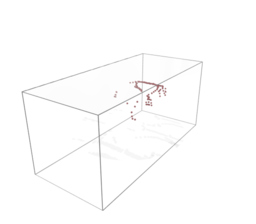
\includegraphics[width=3.75cm,trim={0.5cm 0 1cm 0.75cm},clip]{gfx/overview_small/points/00017}
    \end{subfigure}
    \begin{subfigure}[t]{0.20\textwidth}
        %\hspace*{-0.75cm}
        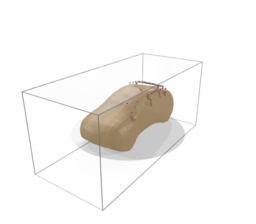
\includegraphics[width=3.75cm,trim={0.5cm 0 1cm 0.75cm},clip]{gfx/overview_small/sdf_points/00017}
    \end{subfigure}\\[-0.1cm]
    \begin{subfigure}[t]{0.5\textwidth}
        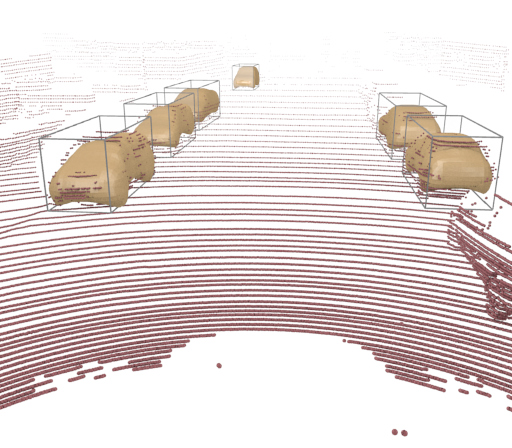
\includegraphics[width=8.25cm,trim={0 8cm 0cm 2cm},clip]{gfx/overview_small/00000}
    \end{subfigure}
    %\vspace*{-4px}
    \caption{{\bf Illustration of the 3D Shape Completion Problem.}
    %On top, we show the Velodyne point cloud of a street scene, annotated with the provided ground truth 3D bounding boxes.
    Top: Given a 3D bounding box and an incomplete point cloud (left, {\color{rred}red}), our goal is to predict the complete shape of the object (right, {\color{rbeige}beige}).
    % missing ground truth shapes.
    %e illustrate an extracted point clouds and the shape completion of our proposed method.
    Bottom: Shape completion results on a street scene from KITTI \cite{Geiger2012CVPR}.
    Learning shape completion on real-world data is challenging due to sparse / noisy observations and missing ground truth.}
    \label{fig:introduction}
    \vspace*{-0.25cm}
\end{figure}